\documentclass{article}
\usepackage{listings}
\usepackage{booktabs}
\usepackage{here}
\usepackage{subcaption}
\usepackage{tikz}
\usepackage{amsmath}
\usepackage{graphicx}
\usepackage{hyperref}


\newcommand{\code}[1]{{\tt #1}}

% decreas margin size
\usepackage[margin=0.7in]{geometry}

\newcommand\blankpage{%
	\null
	\thispagestyle{empty}%
	\addtocounter{page}{-1}%
	\newpage}

\title{
	\normalfont\normalsize
	\textsc{Data Analytics (2024-25)\\
	Universit\`a della Svizzera italiana}\\
	% \vspace{2pt}
	\rule{\linewidth}{0.5pt}\\
	% \vspace{5pt}
	{\huge College network\\
	\small Course Assignment N.13}\\
	% \vspace{5pt}
	\rule{\linewidth}{1pt}\\
	\vspace{5pt}
}

\author{
	Paolo Deidda (\text{paolo.deidda@usi.ch}) \\ 
	Andrea Luca Perugini (\text{andrea.perugini@usi.ch})\\
	\url{https://github.com/USI-Projects-Collection/DA-College_network.git}
	}


\begin{document}
\maketitle

\tableofcontents

\newpage

\section*{Introduction}
This document outlines the structure of the analysis on a dataset of private messages exchanged on a UC Irvine social network.\\

To run the code and reproduce the figures or outputs, please refer to the \texttt{README.md} file for setup and execution instructions.

\section{Data Analysis}
\section{Data Analysis}

\subsection{Setup and Data Loading}
We utilized a dataset provided by the University of California, Irvine, comprising private messages exchanged among users within an online social network. The dataset includes 1899 unique nodes (users) and 59835 edges (messages). The data was loaded into a pandas DataFrame and preprocessed by converting timestamps from Unix time to readable datetime formats, facilitating temporal analysis.

\subsection{Data Exploration}

\subsubsection{Basic Statistics}
The dataset consists of 1899 unique users exchanging messages, resulting in 59,835 interactions. We computed essential statistics:

Total number of users (nodes): 1899

Total number of messages (edges): 59,835

Time span of data collection was determined by inspecting the minimum and maximum timestamps, indicating active periods of communication.

\subsubsection{Message Frequency Over Time}
To explore message distribution over time, messages were grouped and counted by day. Figure 1 clearly demonstrates peaks and troughs, possibly corresponding to academic activities or social events influencing user interactions. This analysis provides insights into temporal dynamics affecting messaging behavior within the network.

\begin{figure}[h]
\centering
% \includegraphics[width=0.8\textwidth]{newplot.png}
\caption{Daily Message Frequency}
\label{fig:message_frequency}
\end{figure}

\subsection{Network Construction}

\subsubsection{Degree Analysis}
We analyzed node degrees to determine connectivity patterns within the network. Nodes with high degrees represent highly interactive users. The degree distribution shown in Figure 2 exhibits a typical scale-free network characteristic, with many users having few interactions and a small subset having numerous interactions, reflecting real-world social networks.

\begin{figure}[h]
\centering
% \includegraphics[width=0.8\textwidth]{degree Distribution.png}
\caption{Degree Distribution}
\label{fig:degree_distribution}
\end{figure}

\subsubsection{Identifying Isolated and One-Way Nodes}
Further examination revealed isolated nodes (users who neither sent nor received messages) and one-way communication patterns (users who either only sent or only received messages). Identifying these nodes helps to understand user engagement and potential network fragmentation.

\subsection{User Analysis}

\subsubsection{Top Senders and Receivers}
We determined users with the highest message activity, distinguishing top senders and receivers. Understanding these roles highlights influential users within the network, possibly indicating user centrality or authority.

\subsubsection{PageRank Centrality}
We calculated PageRank scores to identify influential nodes based on network interactions. High PageRank scores correspond to users frequently contacted by others, emphasizing their significance within the social structure.

\subsubsection{Edge Reciprocity}
Edge reciprocity was analyzed to assess mutual interactions. High reciprocity indicates robust two-way communication, suggesting deeper social connections among users.

\subsection{Temporal Analysis}

\subsubsection{Messages by Weekday}
Analyzing message frequency by weekdays (Figure 3), we observed a clear pattern showing increased messaging during weekdays, which could be aligned with student schedules and reduced activity during weekends.

\begin{figure}[h]
\centering
% \includegraphics[width=0.8\textwidth]{weekday.png}
\caption{Messages by Weekday}
\label{fig:messages_weekday}
\end{figure}

\subsubsection{Top User Activity Analysis}
The hourly activity of top users was analyzed (Figure 4), revealing peak interaction times, which could indicate user availability or preferred communication periods. Such insights can guide future studies on user behavior or network usage patterns.

\begin{figure}[h]
\centering
% \includegraphics[width=0.8\textwidth]{hour.png}
\caption{Hourly Activity of Top Users}
\label{fig:hourly_activity}
\end{figure}



\newpage

\section{Netwrok Analysis}
\subsection{Network Structure Analysis}
\label{sec:network_structure}

The network architecture exhibits key social network characteristics. The calculated \textbf{graph density} is \texttt{0.0056}, confirming a sparse structure typical for such networks where most potential connections are absent. Despite sparsity, analysis of \textbf{weakly connected components (WCCs)} reveals high overall connectivity, with a single giant component encompassing 1893 nodes (over 99.6\% of users), facilitating potential information diffusion.

Considering message directionality (Figure~\ref{fig:scc_visualization}), the \textbf{strongly connected components (SCCs)} analysis identified 601 components, dominated by a large core of 1294 users ($\approx$ 68\%) capable of reciprocal communication. The numerous smaller components highlight a significant periphery, indicating a distinct core-periphery structure critical to information flow dynamics.

Local structure analysis shows moderate \textbf{unweighted clustering} (\texttt{0.087}), suggesting inherent social grouping beyond random chance. However, the \textbf{weighted clustering coefficient} (using message counts) is markedly lower (\texttt{0.0018}). This significant difference implies that while structural triads are present, the intensity of communication within these local groups is often unevenly distributed.


\begin{figure}[h!]
    \centering
    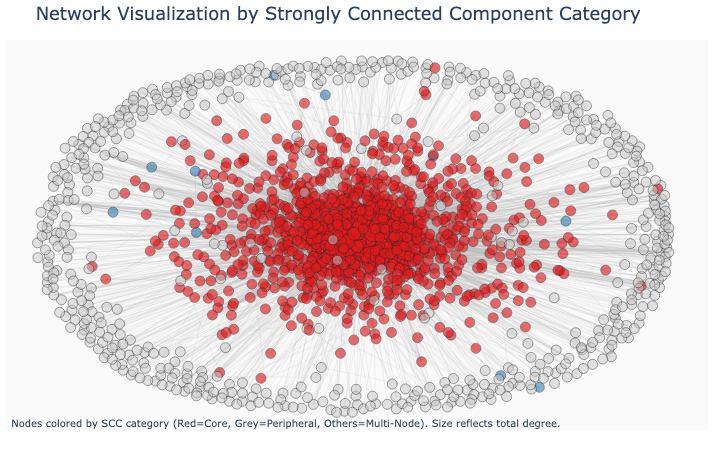
\includegraphics[width=0.9\textwidth]{../scc.png}
    \caption{Network visualization highlighting Strongly Connected Components (SCCs). Nodes coloured by SCC category (Red: Core; Grey: Peripheral; Others: Multi-Node SCCs). Size reflects degree.}
    \label{fig:scc_visualization}
\end{figure}

\subsection{Expanded Centrality Analysis}
\label{sec:centrality_analysis}

Beyond degree and PageRank (Section 1.4), \textbf{Eigenvector Centrality} and \textbf{Betweenness Centrality} provide further insights into node influence and structural roles.

Eigenvector centrality highlights influence via connections to other influential nodes. Top users like \texttt{User 1624} (score $\approx$ 0.47) and \texttt{User 398} ($\approx$ 0.30) demonstrate high influence despite not having top degrees, indicating strategic positioning. Others, like \texttt{User 105} ($\approx$ 0.27), combine high Eigenvector scores with high out-degree and prominence in other rankings.

Betweenness centrality identifies crucial network brokers. Top users \texttt{User 323} ($\approx$ 0.12), \texttt{User 1624} ($\approx$ 0.08), and \texttt{User 105} ($\approx$ 0.08) score highly, reinforcing their central and bridging roles suggested by other measures. The appearance of other high-degree/PageRank users (like \texttt{User 32}, \texttt{User 103}) in the top 10 for Betweenness indicates that popular users can also be important intermediaries.

Analysis of \textbf{Spearman rank correlations} reveals strong positive associations between all centrality measures (most $\rho > 0.7$). In-degree shows particularly high correlation with PageRank ($\rho \approx 0.93$) and Eigenvector ($\rho \approx 0.90$). Betweenness centrality displays slightly weaker, yet still strong, correlations ($\rho \approx 0.72 - 0.81$), suggesting it captures the most distinct structural aspect (brokerage). Overall, these strong correlations indicate that different facets of importance (popularity, influence via connections, brokerage) are significantly intertwined in this network.
\subsection{Network Patterns: Degree Correlation and Activity Symmetry}
\label{sec:degree_patterns}

Examining network mixing patterns, the \textbf{degree assortativity coefficient} was \texttt{-0.1375}. This negative value indicates \textbf{disassortativity}: high-degree users tend to connect with low-degree users, suggesting a hub-and-spoke structure rather than interconnected cores of highly active users.

In contrast to this network-level pattern, individual user activity shows symmetry. A strong positive \textbf{Pearson correlation ($\rho \approx 0.83$)} exists between user in-degree and out-degree, meaning users receiving many messages typically also send many. Thus, while the network structure promotes connections between different activity levels, highly engaged individuals tend to be active communicators in both directions.


% \begin{figure}[h!]
%     \centering
%     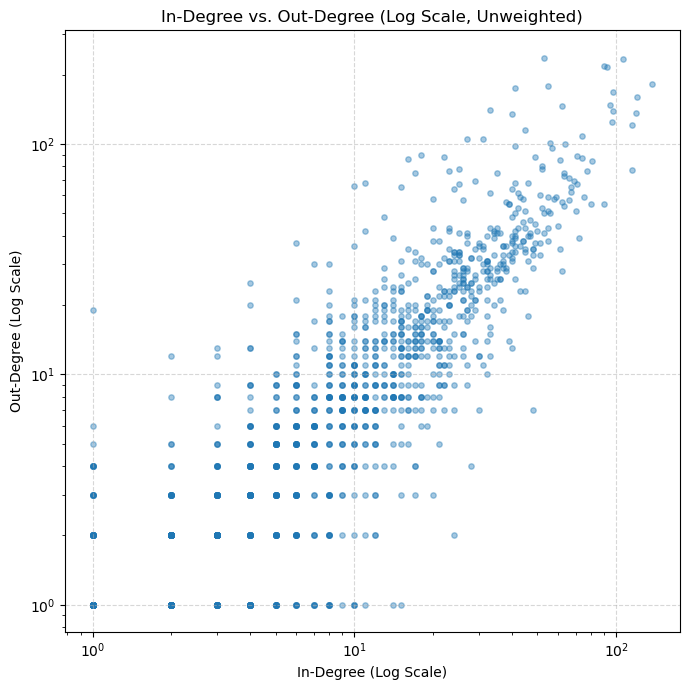
\includegraphics[width=0.7\textwidth]{../inoutdegree.png}
%     \caption{Scatter plot of user in-degree vs. out-degree. The strong positive correlation ($\rho \approx 0.83$) indicates symmetry in individual user activity.}
%     \label{fig:in_out_corr}
% \end{figure}

\subsection{Community Structure}
\label{sec:community_structure}

To uncover meso-scale organization, we applied the \textbf{Louvain algorithm} for community detection. The analysis partitioned the network into \textbf{16 distinct communities} with a \textbf{modularity score} of approximately \texttt{0.3607}. This modularity value indicates a meaningful, albeit imperfect, community structure significantly better than random partitioning.

The detected communities exhibit considerable heterogeneity. Sizes range from large groups (e.g., Community 9: 361 nodes, Community 2: 305 nodes) down to three 2-node communities (likely isolated pairs). Internal structure also varies; the largest communities tend to be internally sparse, while some smaller communities show higher internal density or higher average internal centrality metrics. This community structure is visualized in Figure~\ref{fig:community_visualization}, illustrating the arrangement and relative sizes of the main groups.


\begin{figure}[h!]
    \centering
    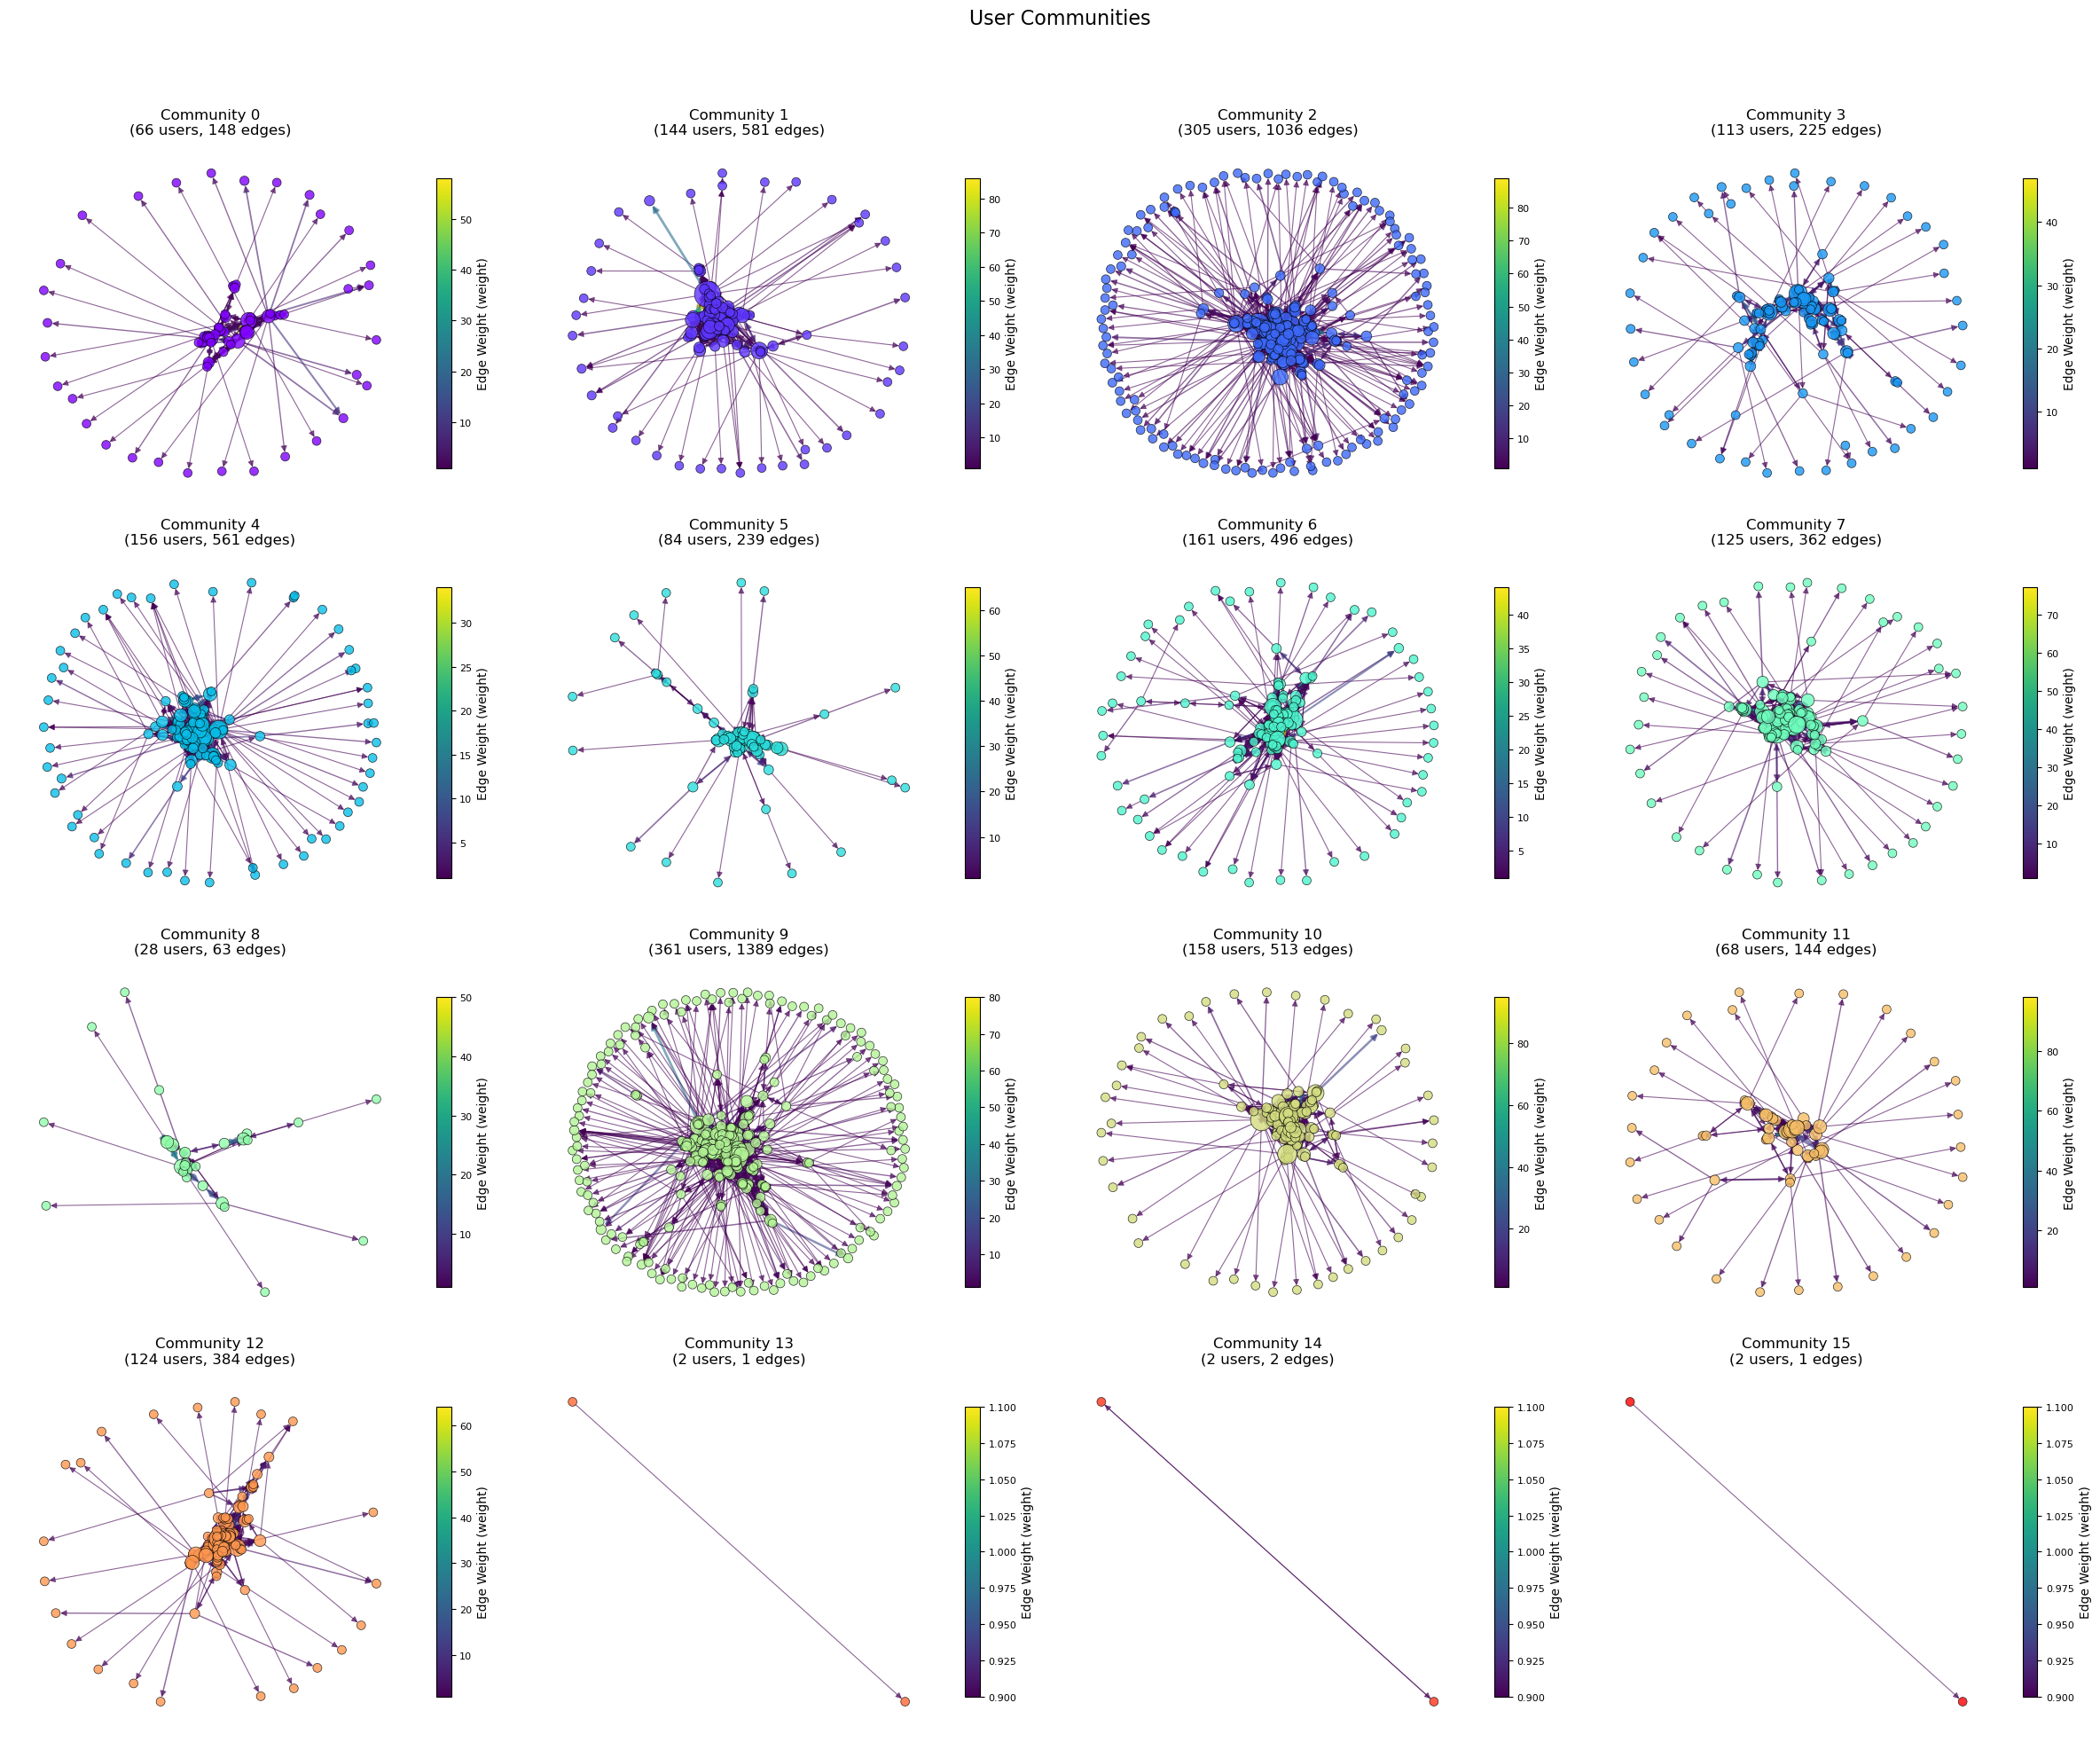
\includegraphics[width=0.9\textwidth]{../communities.png}
    \caption{Network visualization with nodes coloured by detected community membership (Louvain algorithm).}
    \label{fig:community_visualization}
\end{figure}

The presence of this discernible community structure provides valuable insights into the social segmentation within the network.



\section{Final Considerations}



\end{document}